\section{Moduł ST\_INTERVAL}
\subsection{Badania literaturowe}
Zadaniem modułu ST\_INTERVAL jest detekcja oraz analiza tzw. odcinków ST w zarejestrowanym sygnale EKG. Pojedynczy odcinek ST jest fragmentem sygnału ograniczonym przez punkt (oznaczany jako $ ST_{on} $) znajdujący się w okolicach końca poprzedzającego go zespołu QRS (zwanego dalej punktem \emph{J}) oraz punkt początkowy fali T (oznaczany jako $ T_{on} $). Analiza kształtu tego obszaru oraz jego położenia względem linii izoelektrycznej elektrokardiogramu pozwala na stwierdzenie wystąpienia u pacjenta schorzeń takich jak niedokrwienie lub zawał mięśnia sercowego. W czasie normalnej pracy serca, odcinek ST przyjmuje kształt linii prostej, równoległej do izolinii sygnału i oddalonej od niej o około 0.1 mV.  Podczas występowania zaburzeń można zaobserwować zmiany położenia odcinka względem izolinii (tzw. depresje i elewacje) oraz jego kształtu (linie proste o zmiennym nachyleniu, krzywe wklęsłe i wypukłe).
\begin{figure}[H]
	\centering
	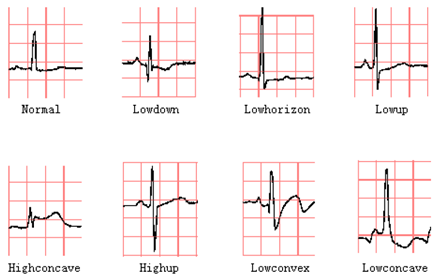
\includegraphics{ST_INTERVAL/img/ST_rodzajeST.png}
	\caption{Rodzaje kształtu odcinka ST [3].}
	\label{fig:ST_rodzajeST}
\end{figure}
Postawiony problem można zatem zdekomponować na następujące zagadnienia:
\begin{enumerate}
	\item Detekcja odcinków ST w sygnale EKG:
	\begin{enumerate}
		\item wyznaczenie punktu $ T_{on} $,
		\item wyznaczenie punktu $ ST_{on} $.
	\end{enumerate}
	\item Analiza kształtu odcinków ST:
	\begin{enumerate}
		\item położenie odcinka względem linii izoelektrycznej,
		\item klasyfikacja kształtu.
	\end{enumerate}
	\item Wykrywanie i ocena epizodów związanych z odcinkami ST wykorzystanie danych o kształcie fragmentów w celu wykrycia potencjalnych zaburzeń.
\end{enumerate}

Najważniejszym zadaniem w pierwszym podproblemie jest poprawne wyznaczenie położenia początku fali T. W dostępnej literaturze można najczęściej spotkać się z algorytmami detekcji bazującymi na transformacji falkowej, wykorzystującymi fakt, iż punkt $ T_{on} $ w większości przypadków jest lokalnym ekstremum sygnału EKG. W opracowaniu [3] zaproponowano analizę zmienności znaku parametrów falkowej dekompozycji sygnału. Odmienne rozwiązanie zostało przedstawione w [1]. Algorytm ten wykorzystuje proste poszukiwanie ekstremów odpowiednio dobranego wskaźnika jakości, bazującego na morfologii (kształcie) fali T.

Wadą metod wykorzystujących falki jest zwiększona złożoność obliczeniowa, a ponadto trudność w doborze parametrów transformacji (tj. wyboru falki-matki, rzędu dekompozycji), w taki sposób, by uwzględniona została każda morfologia fali T. Algorytm bazujący na optymalizacji wskaźnika jakości wykorzystuje znacznie prostsze metody obliczeniowe, dodatkowo w jego konstrukcji uwzględniona została informacja o kształcie fali T, co pozwala na dokładniejszą detekcję pożądanego punktu. Założeniem rozważanych metod jest operowanie na zaszumionym sygnale EKG, stąd w każdej z nich znajduje się pewna forma filtracji (poprzez średnią kroczącą lub w wyniku transformacji falkowej).

Intuicyjna metoda klasyfikacji kształtu odcinka ST opisana została w pracy [2]. Opiera się ona na aproksymacji analizowanego fragmentu dwoma prostymi, umożliwiając jednoczesne wyznaczenie położenia oraz morfologii ST.

\subsection{Koncepcja proponowanego rozwiązania}
Wyznaczenie punktu $ T_{on} $ odbywa się poprzez analizę odcinków znajdujących się pomiędzy punktami $ J $ oraz $ T_{end} $ (koniec fali T). Odpowiedni dobór przedziału poszukiwania ogranicza wpływ morfologii pozostałych zespołów (QRS, P) w sygnale EKG.

Punkt $ T_{on} $ można wyznaczyć poprzez poszukiwanie ekstremów wskaźnika jakości $ A_k $, opierającego się na morfologii fali T [1]. Formuła ta wyznacza dla każdego rozważanego punktu w badanym obszarze wartość stanowiącą analogię pola powierzchni pod sygnałem EKG w oknie przesuwnym o szerokości w próbek, rozpoczynającym się badaną próbką k oraz ograniczonego od dołu wartością tej próbki, co ukazane jest na rysunku \ref{fig:ST_wskaznikAK}.
\begin{equation}
	A_k = \sum_{j=k}^{k+w-1} \left( s_j-\bar{s}_k \right)
\end{equation}
Gdzie:\\
$ k \in \left[ k_a, k_b \right], \; k_a=Q_{end}, \; k_b=T_{end} $ - przyjęty obszar detekcji ST,\\
$ s_i $ - wartość sygnału EKG w i-tej próbce,\\
$ w $ - szerokość okna analizy.\\

Wskaźnik wprowadza także prostą filtrację sygnału (wartość $ \bar{s}_k $), poprzez zastosowanie średniej w ruchomym oknie o szerokości $ 2p $:
\begin{equation}
	\bar{s}_k = \frac{1}{2p+1} \sum_{j=k-p}^{k+p} s_j
\end{equation}
Gdzie:\\
$ p $ - połowa szerokości okna uśredniającego.
\begin{figure}[H]
	\centering
	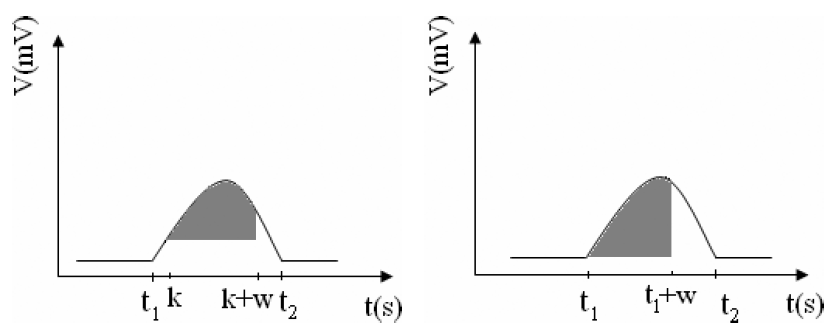
\includegraphics[width=1\textwidth]{ST_INTERVAL/img/ST_wskaznikAK.png}
	\caption{Graficzna interpretacja wskaźnika $ A_k $ [1].}
	\label{fig:ST_wskaznikAK}
\end{figure}
W przypadku analizy nominalnego obszaru zawierającego odcinek ST (linia prosta równoległa do izolinii) oraz falę T (krzywa wypukła), ekstrema wskaźnika $ A_k $ znajdują się w punkcie początkowym fali T (maksimum) oraz jego szczycie (minimum). Wyznaczenie obydwu punktów ekstremalnych $ k' $ oraz $ k'' $ jest konieczne w celu uwzględnienia innych morfologii tej fali (wklęsłości, dwubiegunowości – zob. rys. \ref{fig:ST_morfologieT2}) [1].
\begin{subequations}
	\begin{align}
	k' = \arg \max_{k_a \leq k \leq k_b} A_k \\
	k'' = \arg \min_{k_a \leq k \leq k_b} A_k
	\end{align}
\end{subequations}

Wybór formuły na wyznaczenie punktu $ T_{on} $ zdeterminowany jest przez parametr $ \lambda $ stanowiący wartość progową „przełączającą” algorytm na odpowiednie morfologie fali T. Jeśli spełniony jest warunek:
\begin{equation}
	\frac{1}{\lambda} < \frac{\left| A_{k'} \right| }{\left| A_{k''} \right| } < \lambda
\end{equation}
to:
\begin{equation}
	T_{on} = \min \left\lbrace k', k'' \right\rbrace 
\end{equation}
w przeciwnym wypadku:
\begin{equation}
	T_{on} = \arg \max_{k \in \left\lbrace k', k'' \right\rbrace } \left| A_k \right| 
\end{equation}
\begin{figure}[H]
	\centering
	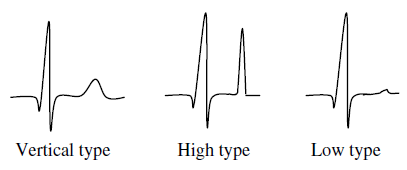
\includegraphics[width=0.62\textwidth]{ST_INTERVAL/img/ST_morfologieT1.png}
	\label{fig:ST_morfologieT1}
\end{figure}
\begin{figure}[H]
	\centering
	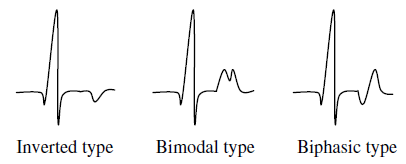
\includegraphics[width=0.62\textwidth]{ST_INTERVAL/img/ST_morfologieT2.png}
	\caption{Morfologie fali T [1].}
	\label{fig:ST_morfologieT2}
\end{figure}
Aby uwzględnić sygnały EKG, w których występuje zjawisko dominacji fali T utrudniające poprawną detekcję krótkich odcinków ST, można wprowadzić następującą modyfikację wskaźnika $ A_k $:
\begin{equation}
	A_k = \sum_{j=k}^{k+w-1} \left( s_j-\bar{s}_k \right)^2
\end{equation}

Wprowadzenie kwadratu do wskaźnika pozwala na zwiększenie wpływu próbek sygnału znacznie oddalonych od linii izoelektrycznej, poprawiając jakość detekcji dla specyficznych przypadków.

Pozycja punktu początkowego fali ST uzależniona jest od szybkości pracy serca [1]. W celu poprawnego wykrycia punktu $ ST_{on} $ konieczne jest obliczenie interwału RT oraz oszacowanie tętna HR osoby badanej. Interwał RT wyznaczany jest jako odległość między punktami $ T_{on} $ i $ R_{peak} $:
\begin{equation}
	RT = T_{on} - R_{peak}
\end{equation}

Tętno można określić na podstawie odległości, w jakiej znajdują się sąsiednie punkty $ R_{peak} $. Posiadając te dane można wyznaczyć punkt $ ST_{on} $:
\begin{equation}
	ST_{on} = R_{peak} + xRT
\end{equation}
Gdzie:
\begin{equation}
	x = 
	\begin{cases}
	0.4		& \text{dla } HR < 100 \\
	0.45	& \text{dla } 100 \leq HR < 110 \\
	0.5		& \text{dla } 110 \leq HR < 120 \\
	0.55	& \text{dla } HR \geq 120
	\end{cases}
\end{equation}

Na podstawie położenia punktów $ J $ oraz $ T_{on} $ można wyznaczyć punkt środkowy $ ST_{mid} $. Odległość tego punktu od linii izoelektrycznej określi odległość $ a_{ST} $ całego odcinka od tej izolinii, która następnie posłuży do oceny położenia fragmentu ST (normalna, depresja, elewacja).
\begin{figure}[H]
	\centering
	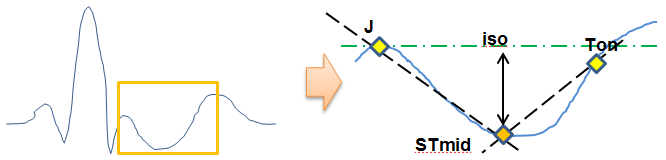
\includegraphics[width=1\textwidth]{ST_INTERVAL/img/ST_aproksymacjaST.png}
	\caption{Aproksymacja odcinka ST prostymi.}
	\label{fig:ST_aproksymacjaST}
\end{figure}
Odcinek ST może być aproksymowany dwoma prostymi łączącymi kolejno punkty $ J $ i $ ST_{mid} $ oraz $ ST_{mid} $ i $ T_{on} $ (rys. \ref{fig:ST_aproksymacjaST}). Kąty nachylenia tych prostych względem izolinii (oznaczane jako $ d_1 $ i $ d_2 $) pozwalają na klasyfikację kształtu odcinka [2].

Wprowadzić można zatem dwa parametry progowe determinujące kształt interwału ST: $ a_{tol} $ (odległość od izolinii), $ d_{tol} $ (kąt nachylenia). Klasyfikacja kształtu zależna od tych parametrów przedstawiona została w tabeli \ref{tab:ST_klasyfikacjaST}. Typowymi wartościami zgodnymi z normami kardiologicznymi [2] są:\\
\[ a_{tol} = 0.1 mV, \; d_{tol} = 35^\circ  \]
\begin{table}[H]
	\centering
	\caption{Klasyfikacja kształtu odcinka ST.}
	\label{tab:ST_klasyfikacjaST}
	\begin{tabular}{|c|c|c|c|c|}
	\hline
	Położenie & Kształt & $ a_{ST} $ & $ d_1 $ & $ d_2 $ \\ \hline
	nominalne	&	-	&	$ \left| a_{st} \right| \leq a_{tol} $	&	-	&	- \\ \hline
	elewacja	&	-	&	$ a_{st} > a_{tol} $					&	-	&	- \\ \hline
	depresja	&	-	&	$ a_{st} < -a_{tol} $					&	-	&	- \\ \hline
	- & horyzontalny & - & $ \left| d_1 \right| \leq d_{tol} $ & $ \left| d_2 \right| \leq d_{tol} $ \\ \hline
	\multirow{3}{*}{-} & \multirow{3}{*}{wzrastający} & \multirow{3}{*}{-} & $ d_1 > d_{tol} $						&	$ d_2 > d_{tol} $ \\ \cline{4-5}
	& & & $ \left| d_1 \right| \leq d_{tol} $	&	$ d_2 > d_{tol} $					\\ \cline{4-5}
	& & & $ d_1 > d_{tol} $						&	$ \left| d_2 \right| \leq d_{tol} $	\\ \hline
	\multirow{3}{*}{-} & \multirow{3}{*}{opadający} & \multirow{3}{*}{-} & $ d_1 < -d_{tol} $						&	$ d_2 < -d_{tol} $ \\ \cline{4-5}
	& & & $ \left| d_1 \right| \leq d_{tol} $	&	$ d_2 < -d_{tol} $					\\ \cline{4-5}
	& & & $ d_1 < -d_{tol} $					&	$ \left| d_2 \right| \leq d_{tol} $	\\ \hline
		-	&	wklęsły		&	-	&	$ d_1 < -d_{tol} $	&	$ d_2 > d_{tol} $	\\ \hline
		-	&	wypukły		&	-	&	$ d_1 > d_{tol}	$	&	$ d_2 < -d_{tol}$	\\ \hline
	\end{tabular}
\end{table}

\subsection{Rezultaty i wnioski}
\subsubsection{Rezultaty testów algorytmu}
Zaimplementowany algorytm w środowisku MATLAB został wielokrotnie przetestowany z różnymi zestawami danych z bazy MIT-BIH oraz European ST-T. Detekcję i analizę odcinków ST przeprowadzono dla pięciu pierwszych uderzeń serca zarejestrowanych na elektrokardiogramie. Wyniki eksperymentów zostały zamieszczone w niniejszym rozdziale wraz z ich interpretacją. Położenie odcinka ST względem linii izoelektrycznej zostało oznaczone w tabelach jako $ a_{st} $, natomiast nachylenia pierwszej i drugiej połowy jako odpowiednio $ d_1 $, $ d_2 $.
Wszystkie testy zostały przeprowadzone przy wykorzystaniu niezmodyfikowanego wskaźnika detekcji (poza przypadkiem zestawu e1304) dla następującego zestawu parametrów:
\[ p = 4, \; w = 30, \; \lambda = 6, \; a_{tol} = 0.15 mV, \; d_{tol} = 35 \]

\subsubsection*{Zestaw danych „100”}
Zestaw ten jest wzorcowym przypadkiem, nie zawierającym jakichkolwiek zaburzeń pracy serca.
\begin{figure}[H]
	\centering
	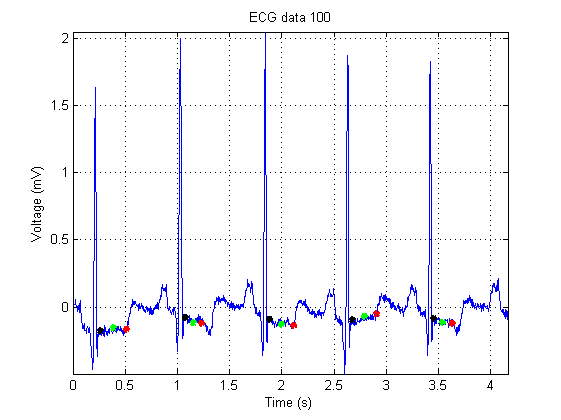
\includegraphics[width=1\textwidth]{ST_INTERVAL/img/ST_zestaw100.png}
	\caption{Rezultaty detekcji dla zestawu „100”.}
	\label{fig:ST_zestaw100}
\end{figure}
Wszystkie charakterystyczne punkty odcinków ST zostały prawidłowo wykryte. Klasyfikacja kształtu i położenia interwałów ST jest zgodna z oczekiwaniami (tabela \ref{tab:ST_zestaw100}).
\begin{table}[H]
	\centering
	\caption{Rezultaty analizy dla zestawu „100”.}
	\label{tab:ST_zestaw100}
	\begin{tabular}{|c|c|c|c|c|c|}
	\hline
	Lp & Typ oczekiwany & Typ wykryty & $ a_{st} [mV] $ & $ d_1 [^\circ] $ & $ d_2 [^\circ] $ \\ \hline
	1	&	Depresyjny horyzontalny	&	Depresyjny horyzontalny	&	-0.155	&	10.426	&	-5.301	\\ \hline
	2	&	Normalny horyzontalny	&	Normalny horyzontalny	&	-0.106	&	-12.113	&	-23.966	\\ \hline
	3	&	Normalny horyzontalny	&	Normalny horyzontalny	&	-0.126	&	-17.299	&	-5.941	\\ \hline
	4	&	Normalny horyzontalny	&	Normalny horyzontalny	&	-0.070	&	12.451	&	5.194	\\ \hline
	5	&	Normalny horyzontalny	&	Normalny horyzontalny	&	-0.099	&	-7.443	&	-14.902	\\ \hline
	\end{tabular}
\end{table}

\subsubsection*{Zestaw danych „105”}
Zestaw 105 jest przypadkiem zawierającym znaczącą ilość depresyjnych i wzrastających odcinków ST, co sugerować może występowanie niedokrwienie mięśnia sercowego pacjenta.
\begin{figure}[H]
	\centering
	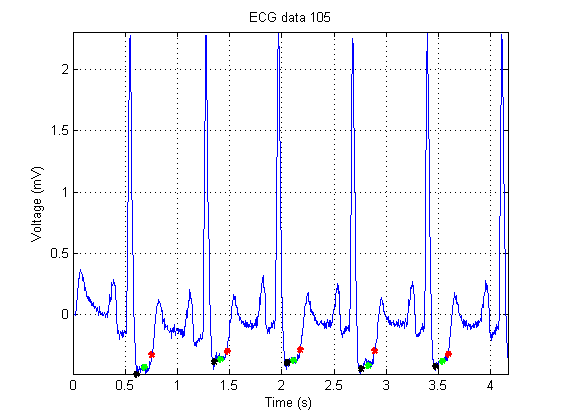
\includegraphics[width=1\textwidth]{ST_INTERVAL/img/ST_zestaw105.png}
	\caption{Rezultaty detekcji dla zestawu „105”.}
	\label{fig:ST_zestaw105}
\end{figure}
Tabela \ref{tab:ST_zestaw105} ukazuje sukces detekcji i klasyfikacji w badanym przypadku.
\begin{table}[H]
	\centering
	\caption{Rezultaty analizy dla zestawu „105”.}
	\label{tab:ST_zestaw105}
	\begin{tabular}{|c|c|c|c|c|c|}
	\hline
	Lp & Typ oczekiwany & Typ wykryty & $ a_{st} [mV] $ & $ d_1 [^\circ] $ & $ d_2 [^\circ] $ \\ \hline
	1	&	Depresyjny wzrastający	&	Depresyjny wzrastający	&	-0.429	&	37.821	&	53.347 \\ \hline
	2	&	Depresyjny wzrastający	&	Depresyjny wzrastający	&	-0.366	&	17.149	&	46.937 \\ \hline
	3	&	Depresyjny wzrastający	&	Depresyjny wzrastający	&	-0.398	&	1.416	&	59.307 \\ \hline
	4	&	Depresyjny wzrastający	&	Depresyjny wzrastający	&	-0.385	&	43.056	&	53.207 \\ \hline
	5	&	Depresyjny wzrastający	&	Depresyjny wzrastający	&	-0.372	&	46.728	&	44.352 \\ \hline
	\end{tabular}
\end{table}

\subsubsection*{Zestaw danych „112”}
Zestaw ten charakteryzuje się występowaniem odcinków ST o morfologii depresyjnej opadającej.
\begin{figure}[H]
	\centering
	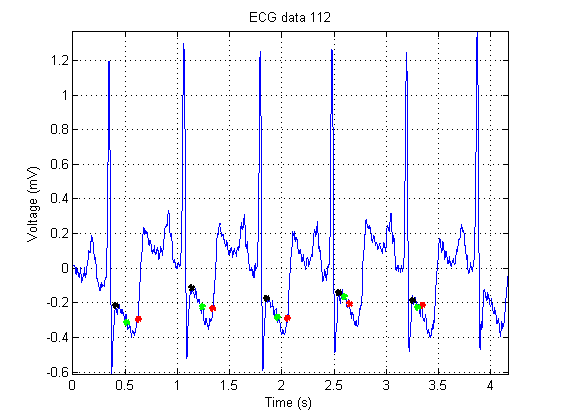
\includegraphics[width=1\textwidth]{ST_INTERVAL/img/ST_zestaw112.png}
	\caption{Rezultaty detekcji dla zestawu „112”.}
	\label{fig:ST_zestaw112}
\end{figure}
Detekcja i klasyfikacja zestawu 112 również zakończyła się pełnym sukcesem (tabela \ref{tab:ST_zestaw112}).
\begin{table}[H]
	\centering
	\caption{Rezultaty analizy dla zestawu „112”.}
	\label{tab:ST_zestaw112}
	\begin{tabular}{|c|c|c|c|c|c|}
	\hline
	Lp & Typ oczekiwany & Typ wykryty & $ a_{st} [mV] $ & $ d_1 [^\circ] $ & $ d_2 [^\circ] $ \\ \hline
	1	&	Depresyjny opadający	&	Depresyjny opadający	&	-0.313	&	-42.806	&	19.021	\\ \hline
	2	&	Depresyjny opadający	&	Depresyjny opadający	&	-0.223	&	-47.684	&	-5.535	\\ \hline
	3	&	Depresyjny opadający	&	Depresyjny opadający	&	-0.282	&	-47.752	&	-17.172	\\ \hline
	4	&	Depresyjny opadający	&	Depresyjny opadający	&	-0.252	&	-40.834	&	24.248	\\ \hline
	5	&	Depresyjny opadający	&	Depresyjny opadający	&	-0.300	&	-45.349	&	0.460	\\ \hline
	\end{tabular}
\end{table}

\subsubsection*{Zestaw danych „103”}
Przypadek został wykorzystany do zbadania skuteczności wykrywania odcinków o morfologii wklęsłej.
\begin{figure}[H]
	\centering
	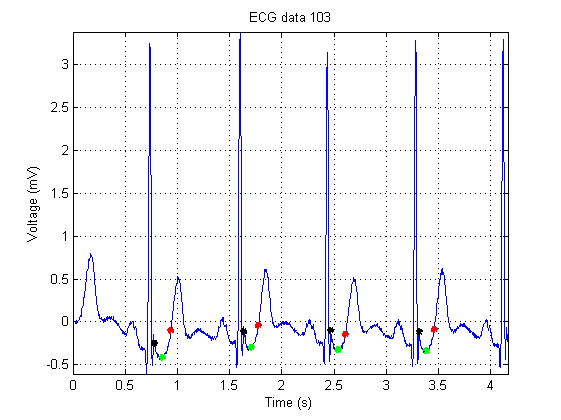
\includegraphics[width=1\textwidth]{ST_INTERVAL/img/ST_zestaw103.png}
	\caption{Rezultaty detekcji dla zestawu „103”.}
	\label{fig:ST_zestaw103}
\end{figure}
Podobnie jak w poprzednich przypadkach, odcinki wykryto i sklasyfikowano poprawnie (tabela \ref{tab:ST_zestaw103}).
\begin{table}[H]
	\centering
	\caption{Rezultaty analizy dla zestawu „103”.}
	\label{tab:ST_zestaw103}
	\begin{tabular}{|c|c|c|c|c|c|}
	\hline
	Lp & Typ oczekiwany & Typ wykryty & $ a_{st} [mV] $ & $ d_1 [^\circ] $ & $ d_2 [^\circ] $ \\ \hline
	1	&	Depresyjny wklęsły	&	Depresyjny wklęsły	&	-0.408	&	-63.650	&	75.819 \\ \hline
	2	&	Depresyjny wklęsły	&	Depresyjny wklęsły	&	-0.293	&	-68.990	&	75.094 \\ \hline
	3	&	Depresyjny wklęsły	&	Depresyjny wklęsły	&	-0.323	&	-73.143	&	69.071 \\ \hline
	4	&	Depresyjny wklęsły	&	Depresyjny wklęsły	&	-0.335	&	-71.824	&	73.186 \\ \hline
	\end{tabular}
\end{table}

\subsubsection*{Zestaw danych „e1304”}
Cechą charakterystyczną elektrokardiogramu \emph{e1304} jest dominacja fali T przy większości uderzeń serca. Powoduje to znaczne zawężenie odcinków ST, utrudniając ich poprawną detekcję.
\begin{figure}[H]
	\centering
	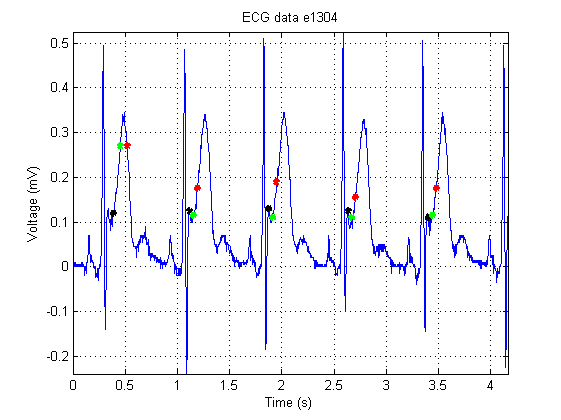
\includegraphics[width=1\textwidth]{ST_INTERVAL/img/ST_zestawE1304.png}
	\caption{Rezultaty detekcji dla zestawu „e1304”.}
	\label{fig:ST_zestawE1304}
\end{figure}
Jak ukazuje tabela \ref{tab:ST_zestawE1304}, każdy z badanych odcinków ST został sklasyfikowany błędnie. Ponadto, większość z nich uznana została jako przypadek bez zaburzeń, co stwarza ryzyko niewykrycia poważnego schorzenia, które wyraźnie sugeruje zwiększona amplituda sygnału EKG (głównie fali T).
\begin{table}[H]
	\centering
	\caption{Rezultaty analizy dla zestawu „e1304”.}
	\label{tab:ST_zestawE1304}
	\begin{tabular}{|c|c|c|c|c|c|}
	\hline
	Lp & Typ oczekiwany & Typ wykryty & $ a_{st} [mV] $ & $ d_1 [^\circ] $ & $ d_2 [^\circ] $ \\ \hline
	1	&	Elewacyjny wypukły	&	Elewacyjny wzrastający	&	0.270	&	65.158	&	-0.000 \\ \hline
	2	&	Elewacyjny wypukły	&	Normalny wzrastający	&	0.115	&	-15.479	&	58.958 \\ \hline
	3	&	Elewacyjny wypukły	&	Normalny wzrastający	&	0.110	&	-28.980	&	65.706 \\ \hline
	4	&	Elewacyjny wypukły	&	Normalny wzrastający	&	0.110	&	-22.557	&	53.471 \\ \hline
	5	&	Elewacyjny wypukły	&	Normalny wzrastający	&	0.115	&	7.326	&	57.051 \\ \hline
	\end{tabular}
\end{table}

\subsubsection*{Zestaw danych „e1304” ze zmodyfikowanym algorytmem}
W celu poprawy analizy badanego przypadku wykorzystana została wspomniana wcześniej modyfikacja algorytmu detekcji.
\begin{figure}[H]
	\centering
	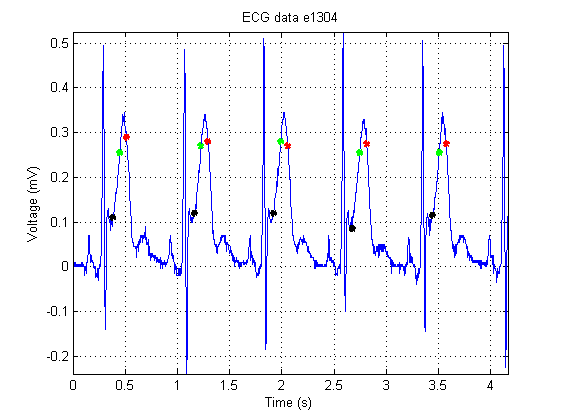
\includegraphics[width=1\textwidth]{ST_INTERVAL/img/ST_zestawE1304mod.png}
	\caption{Rezultaty detekcji dla zestawu „e1304” po modyfikacji algorytmu.}
	\label{fig:ST_zestawE1304mod}
\end{figure}
Po wprowadzeniu modyfikacji otrzymany został częściowo poprawny wynik analizy (tabela \ref{tab:ST_zestawE1304mod}). Położenie każdego z odcinków zostało prawidłowo rozpoznane jako elewacyjne, natomiast niewłaściwie określony został kształt. Mimo błędu, wyniki sugerują zaburzenie pracy serca w przeciwieństwie do rezultatów uzyskanych dla podstawowej wersji algorytmu.
\begin{table}[H]
	\centering
	\caption{Rezultaty analizy dla zestawu „e1304” po modyfikacji algorytmu.}
	\label{tab:ST_zestawE1304mod}
	\begin{tabular}{|c|c|c|c|c|c|}
	\hline
	Lp & Typ oczekiwany & Typ wykryty & $ a_{st} [mV] $ & $ d_1 [^\circ] $ & $ d_2 [^\circ] $ \\ \hline
	1	&	Elewacyjny wypukły	&	Elewacyjny wzrastający	&	0.255	&	65.308	&	28.715	\\ \hline
	2	&	Elewacyjny wypukły	&	Elewacyjny wzrastający	&	0.270	&	66.038	&	8.531	\\ \hline
	3	&	Elewacyjny wypukły	&	Elewacyjny wzrastający	&	0.280	&	66.538	&	-8.531	\\ \hline
	4	&	Elewacyjny wypukły	&	Elewacyjny wzrastający	&	0.255	&	67.780	&	16.699	\\ \hline
	5	&	Elewacyjny wypukły	&	Elewacyjny wzrastający	&	0.255	&	64.537	&	16.699	\\ \hline
	\end{tabular}
\end{table}

\subsubsection{Weryfikacja poprawności implementacji w C++}
Na podstawie algorytmu zbudowanego w środowisku MATLAB utworzona została implementacja w języku C++ z wykorzystaniem bibliotek Qt. Ze względu na odmienne metodyki tworzenia programów w tych środowiskach, przydatna okazuje się automatyczna weryfikacja poprawności działania modułu.
Do badania zgodności implementacji w C++ z algorytmem wzorcowym wykorzystano mechanizm testów automatycznych, które udostępnia środowisko Qt – QT\_TEST. Pozwala on na utworzenie wyspecjalizowanego programu, którego zadaniem jest weryfikacja poprawnego funkcjonowania wybranej części projektu (tzw. \emph{unit tests}).
\begin{figure}[H]
	\centering
	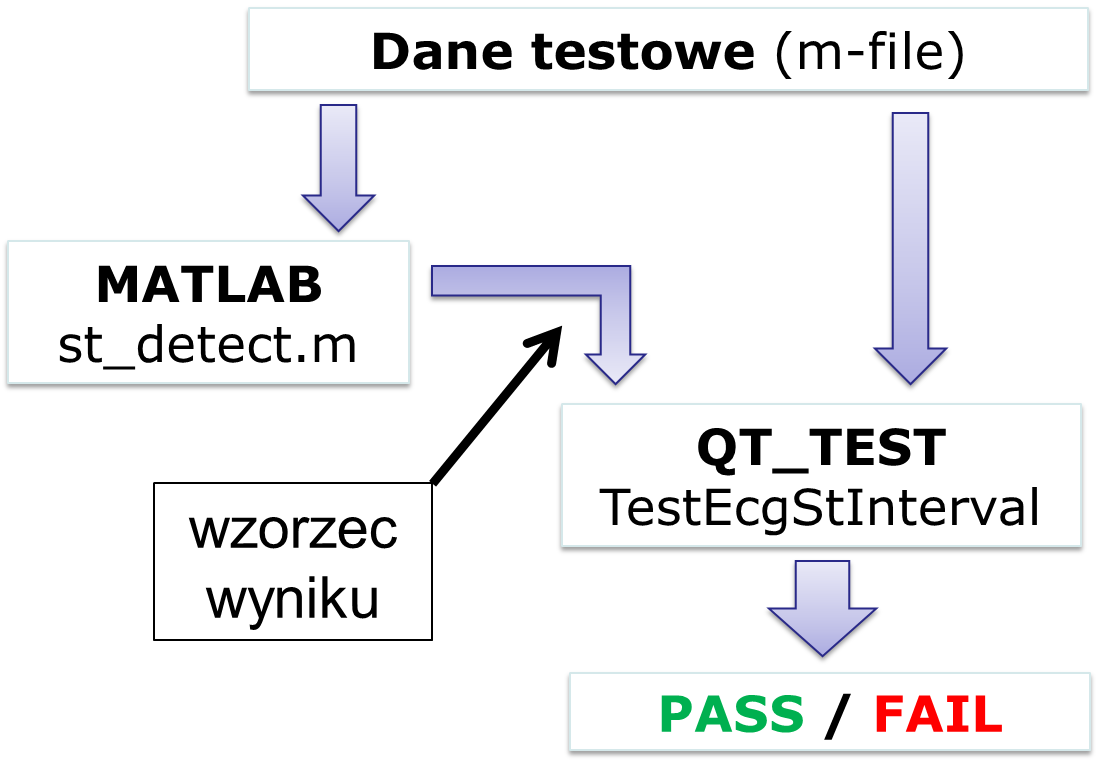
\includegraphics[width=0.6\textwidth]{ST_INTERVAL/img/ST_weryfikacja.png}
	\caption{Przepływ danych testowych w procedurze weryfikacji.}
	\label{fig:ST_weryfikacja}
\end{figure}
Utworzone testy automatyczne wykorzystują ten sam zestaw danych wejściowych, co implementacja w środowisku MATLAB, gdzie generowane są także wzorce poprawnych wyników analizy (rys. \ref{fig:ST_weryfikacja}). Każdy z przypadków testowych przeprowadzany jest według poniższej procedury:
\begin{itemize}
	\item weryfikacja liczby wyników analizy,
	\item weryfikacja klasyfikacji pozycji interwałów ST,
	\item weryfikacja klasyfikacji kształtów ST,
	\item weryfikacja punktów brzegowych i środkowych interwałów.
\end{itemize}

Badanie poprawności detekcji punktów brzegowych i środkowych przeprowadzane jest z zadaną tolerancją, gdyż m.in. ze względu na różnice w błędach obcięcia i zaokrąglenia między C++ a MATLAB pozycje tych punktów mogą się minimalnie przesunąć.

W ramach eksperymentów opisana procedura testowania została przeprowadzona dla czterech zestawów danych: 100, 103, 105, 112 (przedstawionych w poprzedniej sekcji). Implementacja w C++ okazała się zgodna z algorytmem wzorcowym. Wyniki testów ukazane są w tabeli 2.1.3.7. Kolejne kolumny tabeli przedstawiają procent zgodności każdego z etapów weryfikacji.
\begin{table}[H]
	\centering
	\caption{Wyniki weryfikacji implementacji w C++.}
	\label{tab:ST_weryfikacja}
	\begin{tabular}{|c|c|c|c|c|}
	\hline
	Zestaw testowy & Zgodność pozycji & Zgodność kształtu & Zgodność punktów brzegowych \\ \hline
	100 & 100\% & 100\% & 100\%	\\ \hline
	103 & 100\% & 100\% & 90\%	\\ \hline
	105 & 100\% & 100\% & 90\%	\\ \hline
	112 & 100\% & 100\% & 100\%	\\ \hline
	\end{tabular}
\end{table}